\subsection{\textit{Destination sequenced distance vector} - DSDV} 
O protocolo DSDV \'e um protocolo de roteamento proativo\cite{gorantala}, baseado no algoritmo de vetor de dist\^ancias, que trabalha requisitando periodicamente, de cada um dos n\'os vizinhos, suas tabelas de roteamento, com a finalidade de mant\^e-las atualizadas. 
Cada n\'o da rede mant\'em uma tabela de roteamento contendo o pr\'oximo salto e o n\'umero de saltos para cada destino alcan\c{c}\'avel. 
As tabelas incluem rotas para todos os n\'os da rede, mesmo que nunca seja necess\'ario enviar pacote para este n\'o. 
Cada n\'o mant\'em apenas uma rota para cada destino.

Os \textit{loops} de rotas podem ocorrer quando informa\c{c}\~oes de roteamento incorretas s\~ao mantidas na rede ap\'os uma troca de topologia. 
Geralmente ocorre quando um n\'o detecta uma queda no enlace com o n\'o vizinho e, antes que consiga propagar sua nova tabela, recebe de outro n\'o informa\c{c}\~ao desatualizada referente \`a conex\~ao interrompida. 
A vantagem principal do DSDV sobre os protocolos baseados em vetor de dist\^ancias tradicionais \'e que ele garante a aus\^encia de \textit{loops}, usando o conceito de n\'umero de sequ\^encia mantido em cada rota. 
O n\'umero de sequ\^encia \'e estabelecido pelo n\'o destino e \'e incrementado a cada novo aviso de rota.
As rotas mais recentes possuem um n\'umero de sequ\^encia maior e s\~ao as mais favor\'aveis. 
Caso os n\'umeros de sequ\^encia sejam iguais, a rota que tiver o menor n\'umero de saltos ser\'a a mais favor\'avel. 
Neste contexto, o uso de n\'umeros de sequ\^encia faz com que o DSDV se adapte melhor para redes de topologia din\^amica como redes \textit{ad hoc}.

\subsubsection{Exemplo de funcionamento do DSDV}
\begin{figure}[H]
	\centering
	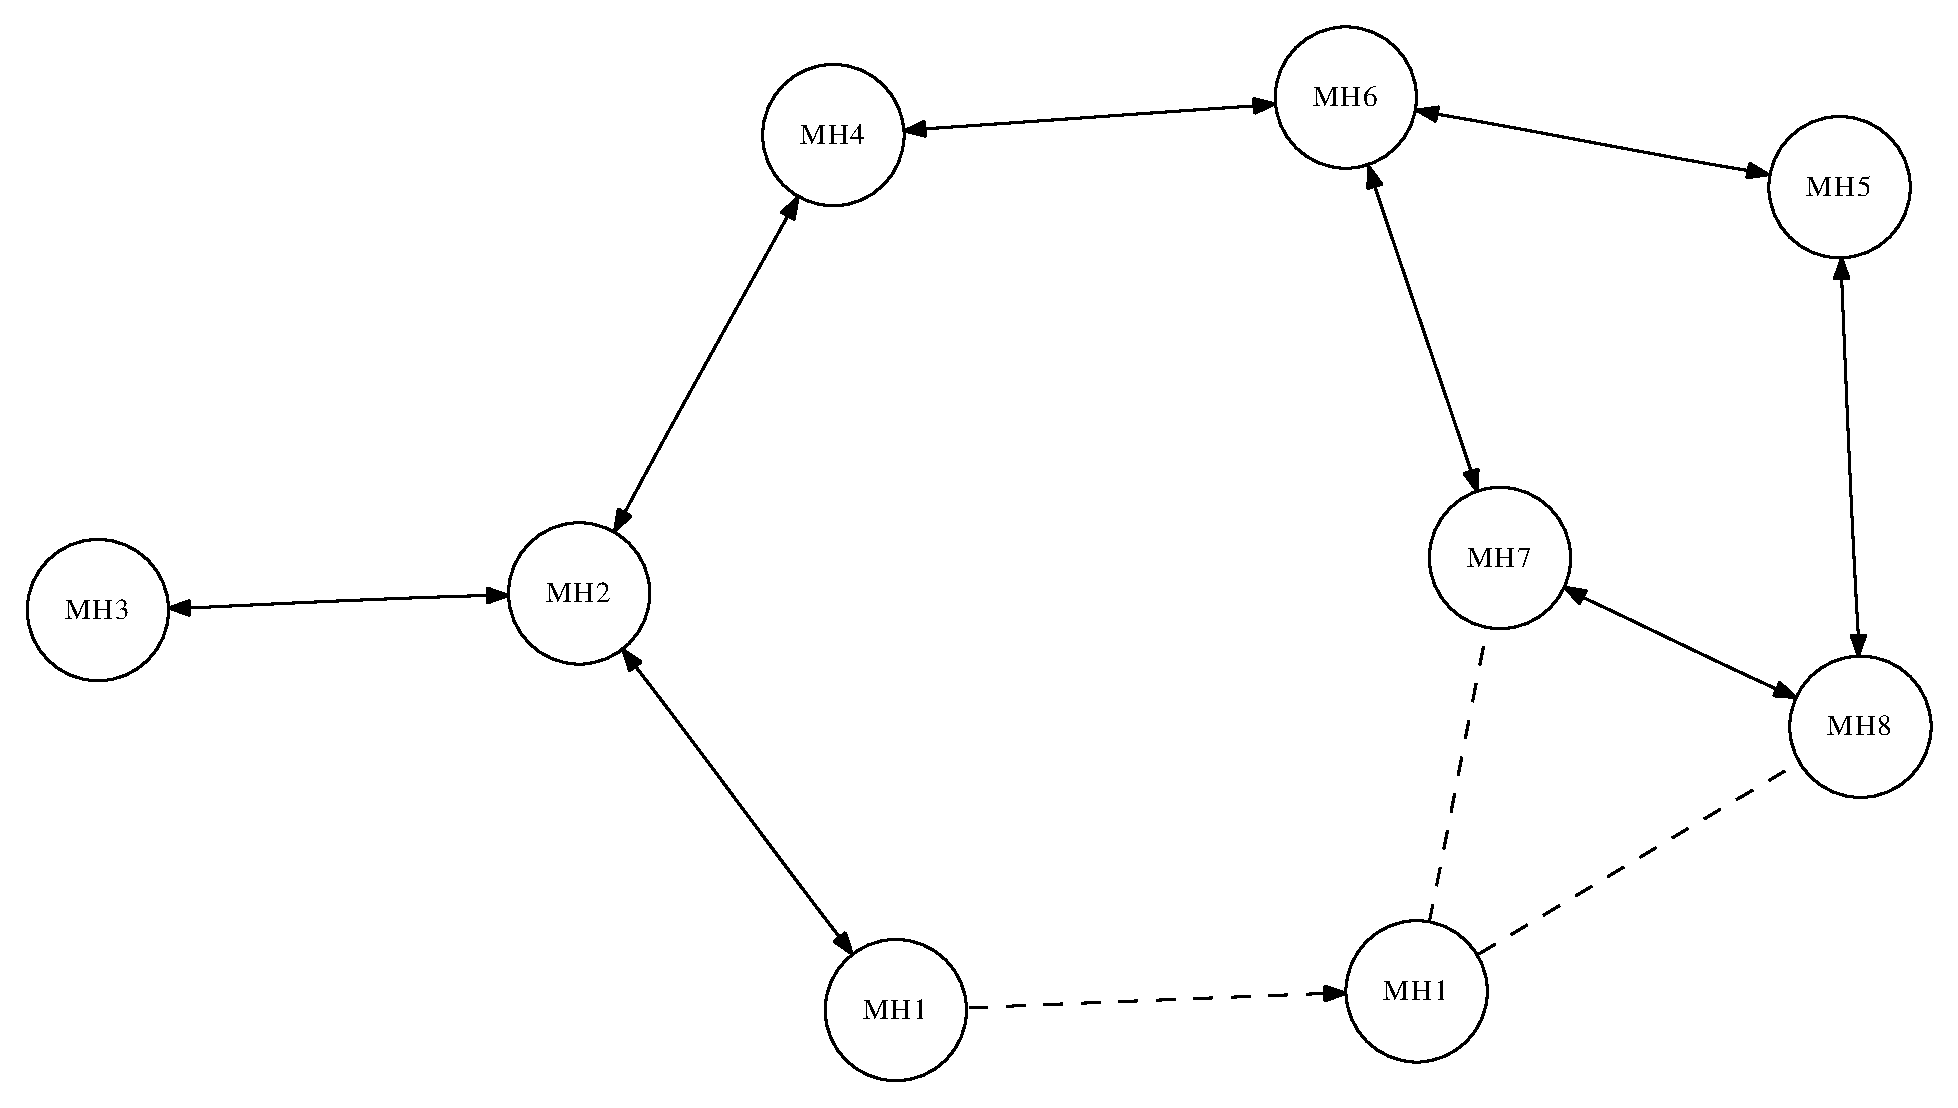
\includegraphics[scale=.5]{dsdvOperation.eps}
	\caption{Exemplo de opera\c{c}\~ ao do DSDV}
	\label{figOpDSDV}
\end{figure}

Considerando a figura \ref{figOpDSDV} acima, possu\'imos 8 hosts em nossa rede. 
N\'os podemos analizar a mudan\c{c}a de roteamento da tabela do MH4 em rela\c{c}\~ao ao movimento do \textit{host} MH1. 
Inicialmente, todos os n\'os anunciam suas informa\c{c}\~oes de roteamento para todos os outros n\'os da rede e, portanto, onde a tabela de roteamento do \textit{host} MH4 inicialmente apresenta o seguinte conte\'udo.

\begin{table}[H]
	\centering
	\caption{Tabela de roteamento do \textit{host} MH4 \cite{pebha}}
	\begin{tabular}{ | l | l | l | l | l | l | }
		\hline
		Destino & Pr\'oximo salto & M\'etrica & N\'umero de sequ\^encia & Install & Informa\c{c}\~ao \\ \hline
		MH1 & MH2 & 2 & S406\_MH1 & T001\_MH4 & Ptr1\_MH1 \\ \hline
		MH2 & MH2 & 1 & S128\_MH2 & T001\_MH4 & Ptr1\_MH2 \\ \hline
		MH3 & MH2 & 2 & S564\_MH3 & T001\_MH4 & Ptr1\_MH3 \\ \hline
		MH4 & MH4 & 0 & S710\_MH4 & T001\_MH4 & Ptr1\_MH4 \\ \hline
		MH5 & MH6 & 2 & S309\_MH5 & T002\_MH4 & Ptr1\_MH5 \\ \hline
		MH6 & MH6 & 1 & S076\_MH6 & T001\_MH4 & Ptr1\_MH6 \\ \hline
		MH7 & MH6 & 2 & S128\_MH7 & T002\_MH4 & Ptr1\_MH7 \\ \hline
		MH8 & MH6 & 3 & S050\_MH8 & T002\_MH4 & Ptr1\_MH8 \\ \hline
	\end{tabular}
	\label{tabRtMH4}
\end{table}

E a tabela de redirecionamento do \textit{host} MH4 esta apresentado da seguinte forma.

\begin{table}[H]
	\centering
	\caption{Tabela de redirecionamento do \textit{host} MH4 \cite{pebha} }
	\begin{tabular}{ | l | l | l | }
		\hline
		Destino & M\'etrica & N\'umero de sequ\^encia \\ \hline
		MH1 & 2 & S406\_MH1 \\ \hline
		MH2 & 1 & S128\_MH2 \\ \hline
		MH3 & 2 & S564\_MH3 \\ \hline
		MH4 & 0 & S710\_MH4 \\ \hline
		MH5 & 2 & S392\_MH5 \\ \hline
		MH6 & 1 & S076\_MH6 \\ \hline
		MH7 & 2 & S128\_MH7 \\ \hline
		MH8 & 3 & S050\_MH8 \\ \hline
	\end{tabular}
	\label{tabRdMH4}
\end{table} 

Por\'em, quando o \textit{host} MH1 move sua localiza\c{c}\~ao para pr\'oximo dos \textit{hosts} MH7 e MH8 como apresentado na figura \ref{figOpDSDV} ent\~ao, o enlace entre MH2 e MH1 vai ser quebrada, resultando em atribui\c{c}\~ao de uma m\'etrica infinita de MH2 para MH1 e o n\'umero de sequ\^encia ser\'a alterado para um n\'umero \'impar na tabela de roteamento em MH2. 
MH2 atualizar\'a essa informa\c{c}\~ao para os \textit{hosts} vizinhos. 
Desde que haja um novo \textit{host} vizinho para MH7 e MH8, eles v\~ao atualizar essa informa\c{c}\~ao nas respectivas tabelas de roteamento e propagam essa nova informa\c{c}\~ao. 
Agora, MH4 receber\'a esta atualiza\c{c}\~ao de informa\c{c}\~ao de MH6, onde MH6 recebe 2 pacotes de informa\c{c}\~oes de diferentes vizinhos para chegar em MH1 com o mesmo n\'umero de sequ\^encia, mas com diferentes m\'etricas. 
A sele\c{c}\~ao da rota ir\'a depender da menor contagem de saltos quando o n\'umero de sequ\^encia \'e o mesmo. 
Agora a tabela de roteamento do MH4 estar\'a dessa maneira.

\begin{table}[H]
	\centering
	\caption{Tabela de roteamento do \textit{host} MH4 depois do movimento do \textit{host} MH1 \cite{pebha}}
	\begin{tabular}{ | l | l | l | l | l | l | }
		\hline
		Destino & Pr\'oximo salto & M\'etrica & N\'umero de sequ\^encia & Install & Informa\c{c}\~ao \\ \hline
		MH1 & MH6 & 3 & S516\_MH1 & T001\_MH4 & Ptr1\_MH1 \\ \hline
		MH2 & MH2 & 1 & S238\_MH2 & T001\_MH4 & Ptr1\_MH2 \\ \hline
		MH3 & MH2 & 2 & S674\_MH3 & T001\_MH4 & Ptr1\_MH3 \\ \hline
		MH4 & MH4 & 0 & S820\_MH4 & T001\_MH4 & Ptr1\_MH4 \\ \hline
		MH5 & MH6 & 2 & S502\_MH5 & T002\_MH4 & Ptr1\_MH5 \\ \hline
		MH6 & MH6 & 1 & S186\_MH6 & T001\_MH4 & Ptr1\_MH6 \\ \hline
		MH7 & MH6 & 2 & S238\_MH7 & T002\_MH4 & Ptr1\_MH7 \\ \hline
		MH8 & MH6 & 3 & S160\_MH8 & T002\_MH4 & Ptr1\_MH8 \\ \hline
	\end{tabular}
	\label{tabNewRtMH4}
\end{table}

E a tabela de roteamento estar\'a nessa maneira.

\begin{table}[H]
	\centering
	\caption{Tabela de redirecionamento do \textit{host} MH4 apos o movimento do \textit{host} MH1 \cite{pebha} }
	\begin{tabular}{ | l | l | l | }
		\hline
		Destino & M\'etrica & N\'umero de sequ\^encia \\ \hline
		MH1 & 3 & S516\_MH1 \\ \hline
		MH2 & 1 & S238\_MH2 \\ \hline
		MH3 & 2 & S674\_MH3 \\ \hline
		MH4 & 0 & S820\_MH4 \\ \hline
		MH5 & 2 & S502\_MH5 \\ \hline
		MH6 & 1 & S186\_MH6 \\ \hline
		MH7 & 2 & S238\_MH7 \\ \hline
		MH8 & 3 & S160\_MH8 \\ \hline
	\end{tabular}
	\label{tabNewRdMH4}
\end{table}

\subsubsection{Vantagens do DSDV}
\begin{itemize}
	\item Livre de \textit{loops} \cite{gorantala}.
	\item Problemas com contagem ao infinito \'e reduzido no DSDV \cite{gorantala}.
	\item Pode-se evitar tr\'afego extra com atualiza\c{c}\~oes incrementais, em vez de atualiza\c{c}\~oes de despejo completo.
	\item Sele\c{c}\~ao de caminho: O DSDV mant\'em somente o melhor caminho em vez de manter v\'arios caminhos para um mesmo destino. Com isso, o espa\c{c}o da tabela de roteamento \'e reduzida.
\end{itemize}

\subsubsection{Limita\c{c}\~ oes do DSDV}
\begin{itemize}
	\item Desperd\'icio do uso da banda na rede devido a propaga\c{c}\~ao desnecess\'aria de informa\c{c}\~oes de roteamento, mesmo se n\~ao houver mudan\c{c}as na topologia da rede \cite{Patel00energyin}.	
	\item O DSDV n\~ao suporta multiplos caminhos de rotas \cite{gorantala}.
	\item \'E dif\'icil determinar um tempo de atraso para a propaga\c{c}\~ao das rotas \cite{heg}.
	\item \'E dif\'icil manter a propaga\c{c}\~ao das tabelas de rotas para uma grande rede. Cada \textit{host} na rede deve manter uma tabela de rotas para propaga\c{c}\~ao. Mas para uma grande rede, isso causaria \textit{overhead}, o qual consome uma maior banda na rede \cite{gorantala}.
\end{itemize}
